%!TEX root = ../template.tex
%%%%%%%%%%%%%%%%%%%%%%%%%%%%%%%%%%%%%%%%%%%%%%%%%%%%%%%%%%%%%%%%%%%%
%% chapter2.tex
%% NOVA thesis document file
%%
%% Chapter with the template manual
%%%%%%%%%%%%%%%%%%%%%%%%%%%%%%%%%%%%%%%%%%%%%%%%%%%%%%%%%%%%%%%%%%%%

\typeout{NT FILE chapter2.tex}%

\chapter{Related Work}
\label{cha:related_work}
In this chapter we examine some topics and techniques that are vital for the work proposal
presented in this document. These topics include \nameref{sec:gossip_protocols}, a dissemination
method, \nameref{sec:wireless_sensor_networks} and of particular interest for applications
devoted to tracking animals, and, lastly, the \nameref{sec:cows}, that explains how the cows behave in herds,
their diet, and its consequences to the plant communities. %TODO: complete
%, and finally, the \nameref{sec:existing_collars},
%where it is discussed some of the existing collars with similar purpose as the proposed to be
%develop during this dissertation.

\section{Gossip Protocols}
\label{sec:gossip_protocols}
%TODO: add a small description

\subsection{History and Overview}
\label{subsec:gossip_history_overview}
%TODO: Citations after gossip protocols??
Gossip protocols, also known as epidemic protocols, as the name indicates, was created
based on how rumors are propagated in social groups. In a gossip protocol, nodes in a
network send the information, randomly, to other nodes in the same network, similar to how a
rumor is spread between members in a social group \cite{Leitao2007}.

Gossip protocols are known as highly scalable and resilient approach to implement reliable
broadcast %TODO: Citation & explain what is a reliable broadcast. 
These protocols are based on every participant propagating their messages collaboratively
throughout all the members of their group.

This process starts when a node desires to propagate some piece of information to the other
members of his network. This node will send his message to \textit{t} nodes, chosen randomly,
(\textit{t} being a parameter called \textit{fanout}, which is better explained in the
Section~\ref{subsubsec:gossip_parameters}). When the receiving nodes receives the message for
the first time, they will do the same as the previous node and resend the message to
\textit{t}, randomly chosen nodes. If a node receives the same message twice, it will discard
it. When this happens, which may occur quite often since the nodes are unaware of which nodes
have already received a message, there is communication redundancy, which while undesirable,
serves the purpose of %!word
omissions (e.g. messages that are not correctly received).

However, since neither node knows who has received each message and who has sent a
message to whom, each node will have to keep a log of all messages that it has already
received, to avoid delivering it multiple times to the application and %!word %!word
to circulate in the network forever.


\subsubsection{Parameters}
\label{subsubsec:gossip_parameters}
Gossip protocols have parameters that should be taken in consideration when using this
class of protocols. The most relevant ones are \cite{Leitao2012}:
\begin{description}
      \item[Fanout:] represents the number of nodes that each node will propagate its message
            to, in each propagating step of the %!word
      \item[Maximum Rounds:] represents how many times a message can be retransmitted. Each
            message has a value of rounds associated to it, starting with zero and adding one
            unit every time a node retransmits the message to a neighbour. When this value
            reaches a maximum round value the message is no longer retransmitted and is simply
            dropped.
\end{description}

Both these parameters demonstrated a clear tradeoff between reliability and redundancy. If
the fanout or the maximum rounds values has a high value the reliability of the protocol will
increase, meaning that the probability that all nodes receive the message increases. However,
the amount of redundancy will also grow, potentially saturating the network, which in extreme
cases can impact negatively the reliability of the dissemination process. The opposite will
occur for low values of each of the parameters.


\subsection{Strategies}
\label{subsec:gossip_strategies}
A Gossip protocol may be executed between pairs of communicating nodes following different
approaches \cite{Karp2000}:
\begin{description}
      \item[Eager push approach:] As soon as a node receive a message for the first time, it
            sends it to \textit{t} randomly selected nodes immediately. This approach consumes
            a great amount of bandwidth, considering it leads to multiple copies of the same
            messages being delivered to each target node.
      \item[Pull approach:] Periodically, nodes inquire each other on new messages they have
            recently receive. If they acquire information about a message they have not
            receive yet, they will request it explicitally from that node. This approach
            leads to higher latency to a message to be received by all nodes, derived from the
            extra round trip needed to obtain a message at each hop of the network.
      \item[Lazy push approach:] When a node receives a message for the first time, it will
            only broadcast to its neighbours a unique identifier of the message, as an example
            a hash of the message. If the neighbour never receives the given identifier, it will
            request the payload of the message. As in the pull approach, there will be a higher
            latency, although somewhat smaller since the transmission of the identifier speeds
            up the propagation of the messages throughout the network.
\end{description}

Besides the previously mentioned differences in latency and bandwidth, there is another
important distinction between the eager push approach and the pull and lazy push approaches.
Considering that the eager push approach sends the entirety of each message immediately after
receiving it, the nodes do not need to maintain a copy of these messages, contrarily to the
other two approaches that may need to resend these messages later. This leads to a higher
memory requirement for these approaches \cite{Leitao2012}.

By combining the approaches studied above, we can get better results, obtaining a better
latency/bandwidth tradeoff. This are two of the studied combined approaches \cite{Carvalho2007}:
\begin{description}
      \item[Eager push and pull approach:] This method is divided between two distinct phases.
            The first phase consists of using the eager push approach to disseminate messages
            straightly to the nodes in the network. The second phase uses the pull approach to
            recover the omissions that might have occurred during the first phase of this
            approach. This strategy reduces the amount of redundancy in comparison with the
            eager push approach, without decreasing its performance. It will, however, lead to
            a higher latency due to the use of the pull phase for recovering from omissions.
      \item[Eager push and lazy push approach:] In this approach eager push is used only to
            propagate messages to a subset of nodes. Then it uses the lazy push approach on
            the remaining subset of nodes to recover from omissions that might occur and
            guarantee the reliability of the dissemination process.
\end{description}


\subsection{Tree-based Approaches}
\label{subsec:gossip_tree_based_approaches}
Tree-based broadcasting methods have a small message complexity, however, they are not
particularly resilient to faults. On the other hand, gossip protocols, as mentioned earlier
in Section~\ref{subsec:gossip_history_overview}, are known for their resilience, but have a
high message complexity \cite{Leitao2007Tree}.

In order to obtain a small message complexity and high reliability, previous approaches have
considered combining both these methods.

With this approach we obtain the nodes organized in a tree structure topology, where each node
knows to whom forward its messages. To achieve this structure we have many approaches, one of
the most popular is to rely on the PlumTree protocol.
\begin{description}
      \item[PlumTree protocol] This protocol uses eager push and lazy push gossip, previously
            explained in the Section~\ref{subsec:gossip_strategies}. It separates the nodes in the
            network in two subsets of randomly selected nodes. The first subset of nodes uses the
            eager push protocol to disseminate the messages, while the other uses the lazy push
            protocol.
            %TODO: explain better how it works
            The links that the eager push method uses to propagate the messages are
            chosen to create a randomized broadcast network that converges to a tree-based
            structure. While the links used during the lazy push gossip are used to ensure the
            reliability of the method when nodes fail and potentially heal the broadcast tree
            when needed \cite{Leitao2007Tree}.
\end{description}

Additionally, in opposition to other dissemination protocols, that rely on tree-based gossip the
connections first made by the eager push propagating will remain until it is detected a failure.
This will allow us to use \Gls{TCP} connections, which will provide extra reliability and
failure detection.


\subsection{Examples}
\label{subsec:gossip_examples}
Throughout the last years there have been proposed numerous gossip-based protocols. During this
section we will discuss some of them:
%TODO: this are overlay networks but it should be dissemination
\begin{description}
      \item[\Gls{Scamp}:] Contrarily to many other gossip-based protocols, with Scamp
            it is proposed that the individual nodes have a randomized partial view of the global
            members in the network, leading to a fully decentralized system. This is quite an
            important advantage for large scale groups, since it requires a significant amount
            of memory and generates a lot of network traffic to maintain the system's overall
            consistency in extensive groups. Additionally, the scalable membership protocol is
            also compelling for its natural increase and reorganization of the partial view of
            the system when new nodes are added to the network. Having this partial view around
            \textit{log n} nodes (being \textit{n} the number of overall nodes in the network)
            \cite{Ganesh2001}.
            %TODO: too vague, missing how it works and proprieties that garantees
      \item[\Gls{NeEM}:] One of the biggest problems in most gossip-based protocols is when the
            network gets congested and, subsequentially, the messages get lost. NeEM
            uses \glsxtrshort{TCP} to disseminate the messages and resolve this problem, with the
            usage of its inherent flow and congestion control mechanisms. In order to maintain
            the protocol's stability, NeEM uses a buffer management technique that
            utilizes different approaches to discard messages on overflow. It also includes the
            knowledge about the messages' types in order to ensure that the buffer retains enough
            space and bandwidth is used to better fit each request \cite{Pereira2003}.
            %TODO: too vague, but is gossip propagation
      \item[\Gls{CREW}:] Is a gossip-based protocol designed to minimize the messages
            dissemination speed. This is acquired by maintaining in cache the information about
            the already established connections, which will reduce the latency of reopening a
            \glsxtrshort{TCP} connection \cite{Deshpande2006}.
            %TODO: too vague
            % TODO: scribe and potentially MON
            %\item[Scribe:] Scribe is a large scale and fully descentralized
\end{description}


\subsection{Gossip Limitations}
\label{subsec:gossip_limitations}
Throughout this Section it has been vastly mentioned the advantages provided by gossip
protocols. Mainly, it was referred the resilience and scalability offered by this approach.
However, as any other protocol, it has its limitations. A few of this are \cite{Birman2007}:
\begin{enumerate}
      \item Fixed maximum message size - gossip protocols have a fixed maximum message size
            which may lead to problems. %* might be untrue
            As an example, if we desire to propagate a message with a larger size than this
            fixed maximum message size, we will have to divide the message into multiple
            segments. When this happens, some of these segments may be lost, since each node
            can only gossip a certain amount of information per %!word
            unit (occasionaly named round), which will increase the number of rounds required
            to deliver a single message to all participants.
      \item Slow rate - the rate of messages exchange in a gossip protocol is typically quite
            low, which can cause some challenges when managing sudden and urgent events. This
            situation might be surpassed by reducing the periodicity of messages exchanges;
            however, this often leads to yet another problem, the increasing of overhead and
            potentially network congestion.
      \item Malicious behaviours and correlated loss patterns - another limitation of gossip
            protocols is that when the nodes behave in a malicious way, intentionally, such as
            disseminating of false information or when nodes malfunction, even if unintentionally,
            gossip protocols can be disrupted, or effectively propagate incorrect information.
\end{enumerate}


\subsection{Discussion}
\label{subsec:gossip_discussion}
Throughout this Section it has been described the fundamental approaches of gossip protocols,
the main strategies, a tree-based approach, some interesting examples of gossip-based methods
and finally their limitations.

This class of protocols is crucial for the development of this dissertation %TODO: why...

Since it is highly scalable and reliable, the gossip protocol will be helpful while dealing
with the propagation of data in a system with over 150 cows. Due to the lack of network
coverage in most of the farm, the information collected from devices on each cow will have to
be communicated to their neighbours until it reaches a point of connection to the management
platform.

The PlumTree approach is quite interesting for addressing some of the challenges in this work
considering that the cows follow a hierarchy just like a tree-based protocol is design to do.
The PlumTree can then mimic the herds' hierarchical system and find the cows that spend more
time in close proximity making sending the information throughout the herd until the user
easier. Unfortunately PlumTree was proposed for wired networks, where devices %!word 
by cows will necessarly communicate via wireless, potentially in an infrastructure %!word
network (ad hoc network) which is %!phrase


\section{Wireless Sensor Networks}
\label{sec:wireless_sensor_networks}

\subsection{Definition}
\label{subsec:wsn_definition}
\Gls{WSN} is a technology with many applications ranging from remote environmental monitorization
to target tracking. These networks are composed by multiple small cheap and low-power sensor
nodes distributed throughout various locations.

Usually, the nodes are scattered in a sensor field, as demonstrated in Figure~\ref{fig:sensor_nodes_in_sensor_fields}.
Individually, each node can perform sensing tasks, which implies:
\begin{itemize}
      \item collecting data, for example, from its surroundings, such as temperature, light,
            humidity, and many other types of data, depending on the types of sensors in the
            device;
      \item process it, using its on-board processor;
      \item and finally, transmit it back to the sink (a node that has the capacity to communicate
            with external devices, such as phones and laptops) by multi-hopping. It eventually
            reaches the end users via internet or a satellite from the %!work 
            sink node \cite{Akyildiz2002}.
\end{itemize}

\begin{figure}[H]
      \caption{Sensor nodes in a sensor field \cite{Akyildiz2002}}
      \centering
      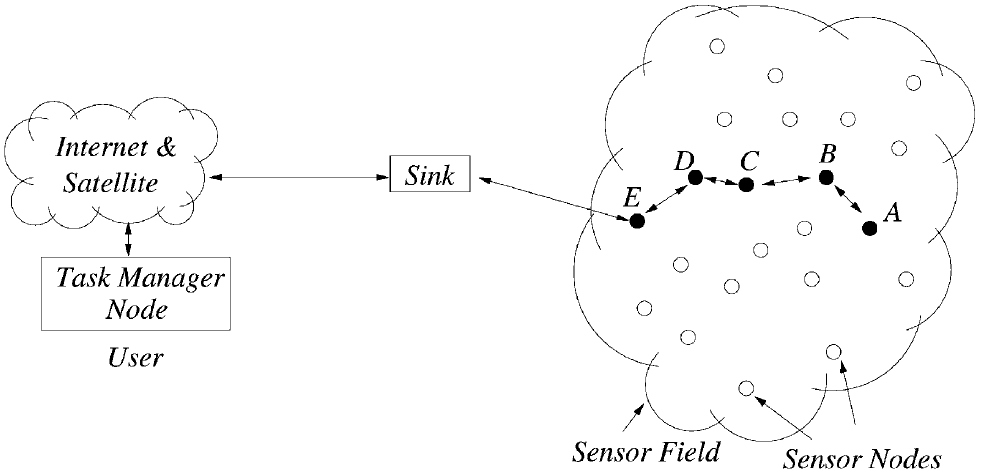
\includegraphics[scale=0.5]{Chapters/Figures/sensor_nodes_in_sensor_fields.png}
      \label{fig:sensor_nodes_in_sensor_fields}
\end{figure}
%TODO: define sink


\subsection{Wireless Technologies}
\label{subsec:wsn_wireless_technologies}
%TODO:


\subsection{Communication Architecture}
\label{subsec:wsn_communication_architecture}
The most common architecture for \glsxtrshort{WSN} follows the OSI model. This model is
composed of five layers: application layer, transport layer, network layer, data link layer
%* seven layers, censi presentation and sensor ?? 
and physical layer, and three cross plane layers: power management plane, mobility management
plane and task management plane, as shown in Figure~\ref{fig:wsn_architecture}.

\begin{figure}[H]
      \caption{\glsxtrshort{WSN} Communication Architecture \cite{Akyildiz2002}}
      \centering
      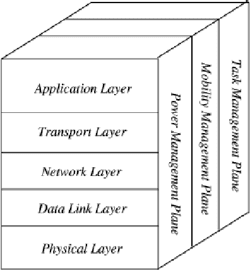
\includegraphics[scale=0.5]{Chapters/Figures/wsn_architecture.png}
      \label{fig:wsn_architecture}
\end{figure}

The five layers above mentioned work together to ensure the data is properly transmitted to
the network, each with a specific functionality \cite{Akyildiz2002, Matin2012}:
\begin{description}
      \item[Application Layer] provides to the end user an interface that he can interact with.
            Depending on the sensing tasks there are various types of application software that can
            be built.
      \item[Transport Layer] ensures the transportation of data in a reliable and orderly manner,
            even if the network suffers disruptions.
      \item[Network Layer] maps to where the data supplied by the transport data should go to
            next.
      \item[Data Link Layer] is responsible for confirming that the data transmitted is
            reliable and the transmission itself is efficient and secure. The main tasks of the
            data link layer are: 1) reducing the data received from the network layer into frames;
            2) find and correct errors in the frames, when possible; otherwise, discard them; 3)
            multiplexing of data streams; 4) \Gls{MAC}
      \item[Physical Layer] addresses the need for a simple but robust modulation, transmission
            and receiving techniques.
\end{description}

The management plane main roles are to include managing the network and optimize the sensor
nodes performance to improve the overall effectiveness of the network, considering the
advantages acquired by all sensor nodes working together. Each of these planes manages
a specific area \cite{Akyildiz2002}:
\begin{description}
      \item[Power Management Plane] manages how the sensor node uses its power, choosing when to
            turn off its receiver to save energy or to keep it from receiving repeated messages. It
            also informs its neighbours when it reaches a low power mode.
      \item[Mobility Management Plane:] keeps track of the sensor nodes neighbours and always
            distinguishes a route back to the user.
      \item[Task Management Plane:] administers the periodicity and schedule that each node needs
            to maintain in order to perform their sensing tasks based on their power dependency and
            task requirements.
\end{description}

\subsection{Network Topologies}
\label{subsec:network_topologies}
There are several different topologies regarding the connection between nodes and their message
exchange routes, as represented in the Figure~\ref{fig:network_topologies} \cite{Lewis2004, Yadav2012}:
\begin{description}
      \item[Star Topology:] all nodes are connected to only one node, the coordinator. This
            means every node will communicate via this central node and every node that requests
            to enter this network will have to send its information to the coordinator, which
            will then send it to the other nodes. The principal limitation of this topology is
            that if the coordinator malfunctions the whole network will fail.
      \item[Ring Topology:] all nodes are equal connected, having no coordinator. Contrarily
            to the star topology, if a single link is broken the whole network will fail.
      \item[Bus Topology:] all nodes broadcast their messages using the bus. Each message
            has a header with the destination address so that every node can see if the message
            is for them or another node. This topology is passive, since the nodes are not
            responsible for retransmitting messages.
      \item[Tree Topology:] similar to the star topology where the coordinator is the tree root, on
            the other hand the nodes at different levels of hierarchy are connected to sub-coordinators
            that lead to the root \cite{Shrestha2007}. In this topology, as in the star topology, if
            the coordinator malfunctions, the whole network will fail. However, differently from
            the star topology, will also have problems if a sub-coordinator fails as it will lead
            to the failure of every subordinate node.
      \item[Fully Connected Topology:] every node is connected to every other node. This will
            lead to a routing problem when dealing with large networks.
      \item[Mesh Topology:] the nodes are generally identical, so the mesh connections are
            commonly referred as peer-to-peer connections. However, even though the nodes are
            generally identical some of them can be assign as coordinators that take additional
            functions and if one of these coordinators stops working, another just takes over his
            work. An interesting aspect of this topology is that the communication can be
            done between any two nodes in close proximity, which makes this topology quite
            robust to the failure of nodes or links, since the messages can use other routes to be
            delivered, and it is quite efficient for large scale networks.
\end{description}

\begin{figure}[H]
      \caption{Network Topologies \cite{Lewis2004}}
      \centering
      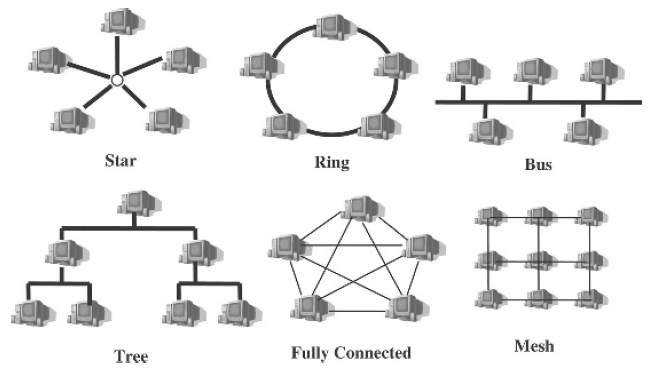
\includegraphics[scale=0.7]{Chapters/Figures/network_topologies.png}
      \label{fig:network_topologies}
\end{figure}

% \subsection{Strategies}
% \label{subsec:wsn_strategies}
% % TODO:
% The WSN have innumerous applications, this idea will be further discussed in the subsequent
% subsection \ref{subsec:wsn_applications}, which will lead to different solutions for each of
% them.

\subsection{Gossip in WSNs}
\label{subsec:gossip_in_wsns}
One of the main purposes of a sensor node is to transmit the data it has collected, via
the sensors, to the sink. The route chosen by these nodes has a significant impact on the
overall operation of the system, therefore various protocols were studied in \cite{Akkaya2005}
to understand which of these would better conduct this task.

As presented previously, in the Section~\ref{sec:gossip_protocol}, during the execution of a
gossip protocol each node only transmits its messages to \textit{t} randomly selected nodes
and not the whole network, as in the flooding protocol. This characteristic ensures that every
node executing a gossip protocol will only have a single copy of the packet to be sent, which
addresses one of the shortcomings of the flooding protocol, the implosion. %TODO: cite and define implosion
However, this will lead to delays in the dissemination of the data which may be an important
factor for some applications of the network.

%TODO: give examples of these protocols in wireless networks

\subsection{Applications}
\label{subsec:wsn_applications}
Due to the fact that the sensor nodes in a \glsxtrshort{WSN} may collect distinct types of
data, based on sensing task and the sensor itself, there are many applications and
subsequentially many are areas of expertise in WSR. These areas may be related to health, the
military, home, environmental, commercial and many more. For this thesis it is more impactful
to learn about some of the applications in the tracking area, per example, \nameref{subsubsection:zebranet}
and \nameref{subsubsection:wireless_tracking}.

\subsubsection{ZebraNet}
\label{subsubsection:zebranet}
One of the most revolutionary applications of \glsxtrshort{WSN} is the ZebraNet, a method
developed to track wildlife, specifically, zebras, for biology research, using a mobile base
station. The ZebraNet collects logged data from tracking collars, transported by the
animals, and afterward it transmits this data back to the researchers. Considering there
is no fixed antennas or cellular telephone service, the protocol uses ad hoc
peer-to-peer routing to transport the data around.

The ZebraNet project focused on addressing some of the problems observed from previous
studies of collecting data from wildlife. One of the main obstacles was using
satellites to transport the data. The process of uploading data to satellites is slow and
power consuming. Moreover, the data download from the satellite to the researchers is
charged by the bit, which restricted the amount of data collected. Furthermore, these
systems used batteries without solar panels, which would eventually end, and had to be
recovered and recharged, losing enormous amounts of data in process \cite{Juang2002}.

Additionally, one of the biggest concerns during the development of this project was the
design limitations. Due to the fact that each node would be transported by an animal,
its weight and size was immediately limited. And since the nodes are difficult to
retrieve, the device had to have a durable battery life \cite{Zhang2004}. Subsequentially,
most of the weight would be occupied by the battery and the GPS, leaving a small
space for the storage, which meant that there were a small space for redundant messages in
this protocol. Lastly, it was crucial to consider the impact of the number and size of data
transmissions required as well as the range of these transmissions.
% TODO: explain in more detail how it works

\subsubsection{Wireless Tracking}
\label{subsubsection:wireless_tracking}
Wireless tracking is an application of \glsxtrshort{WSN} widely used for wildlife research,
since it allows the remote monitorization of moving objects, or in this particular case,
animals.

To track an object the sensor nodes detect its location and sends this information to the end
user. There are mainly two options to accomplish this: using only a single node or multiple
nodes working collaboratively. Using multiple nodes is an overall better choice, since it leads
to higher accuracy and lower power consumption comparably to using a single node \cite{Ez2016}.

To achieve an efficient target tracking performance it was developed countless methods,
contemplating the challenges existent with using \glsxtrshort{WSN}, discussed furthermore in
the Section~\ref{subsec:wsn_limitations}. These methods take into account the continuous
localization of mobile nodes over time, determine their speed at each moment and often use
their known former localization to improve accuracy \cite{Kumar2017}.

There are three main types of target tracking approaches according to \cite{Ramya2012} authors:
\begin{enumerate}
      \item Hierarchical Networks - the nodes communication follows a mesh based topology,
            thoroughly explain in the Section~\ref{subsec:network_topologies}, using multihop
            radio connectivity. This enables the communication between two nodes that are not
            in a direct communication range, by forwarding their messages through other nodes in
            their ranges until the messages achieve their final destination.
            \begin{enumerate}
                  \item Tree Based Target Tracking - the nodes are organized in a hierarchical
                        tree structure or represented as a graph, where the vertices represent the
                        nodes and the edges the connections between two nodes that can communicate
                        directly. The node
                  \item Cluster Based Target Tracking -
                        \begin{enumerate}
                              \item Static Clustering -
                              \item Dynamic Clustering -
                              \item Space-Time Clustering -
                        \end{enumerate}
                  \item Mobicast Message Based Tracking -
                  \item Hybrid Method -
                  \item Activation Based Method -
            \end{enumerate}
      \item Peer-to-peer Networks -
      \item Other Network -
\end{enumerate}


%TODO: mirage de aves? e ygsodresi
% In a target tracking application, the sensor nodes which can sense the target at a particular 
% time are kept in active mode while the remaining nodes are to be retained in inactive mode so 
% as to conserve energy until the target approaches them. To continuously monitor mobile target, 
% a group of sensors must be turned in active mode just before target reaches to them. This 
% group of active sensors varies depending on the velocity of moving target and schedule from 
% cluster head.\cite{Ramya2012}



% Nonetheless, every node being constantly in a state of alert,
% detecting the movement of the object and sending control data at the same time, will consume
% an enormous amount of energy. It was, however, developed a technique that dynamically allocates
% resources, the \Gls{CSIP} \cite{Zhao2003}.



\subsection{Limitations}
\label{subsec:wsn_limitations}
There are multiple limitations that need to be considered while creating a \glsxtrshort{WSN}
\cite{Akyildiz2002, Matin2012}:
\begin{itemize}
      \item \textbf{Fault Tolerance} - the sensor nodes can fail due to lack of power, hardware
            problems or physical damage, contemplating the harsh environments they are exposed to
            and their own fragility. Therefore, the protocols employed in the sensor network
            need to possess the ability to quickly identify any malfunctions and possess the
            robustness necessary to sustain the network's overall functionality, even with a large
            number of failures.
      \item \textbf{Scalability} - the sensor networks might have hundred, thousand or even
            millions of nodes. Therefore, the protocols employed in these sensor networks need to
            be scalable to these levels and maintain a tolerable efficiency level.
      \item \textbf{Production Costs} - since a sensor network is composed by a large number of
            nodes it is important that this value is quite small, ideally much lower than US\$1.
      \item \textbf{Hardware Contraints} - a sensor node is usually constituted by a sensing
            unit, a processing unit, a transmission unit and a power supply, as represented in
            Figure~\ref{fig:sensor_components}. Additionally, it may be necessary to add some
            extra components, as per example a localization system. These need to consider the
            extra costs, the power consumption it will lead to and finally, the space available
            in the node.
            \begin{figure}[H]
                  \caption{Sensor node typical architecture \cite{Akyildiz2002}}
                  \centering
                  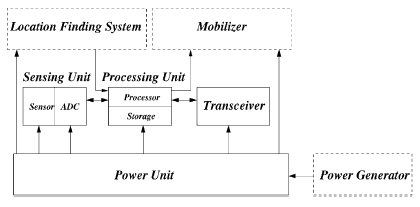
\includegraphics[scale=1]{Chapters/Figures/sensor_components.png}
                  \label{fig:sensor_components}
            \end{figure}
      \item \textbf{Sensor Network Topology} - energy consumption is the main obstacle regarding
            \glsxtrshort{WSN} performance and efficiency. To combate this problem it has been
            researched numerous algorithms, protocols and techniques, being topology maintenance
            one of the most important to reduce energy consumption.
      \item \textbf{Transmission Media} - most communication networks use \Gls{RF} to connect
            the nodes wirelessly. There are, however, other ways of connection, using optical or
            infrared communication. Both optical and infrared communication require a line of
            sight between the sender and the receiver. However, the infrared communication has
            the advantage of being less affected by other electonic devices.
      \item \textbf{Power Consumption} - derived from the node size and the, sometimes,
            impossibility to recharge its battery, the lifetime of a node depends entirely
            on the management of this resource. Therefore, it is of the utmost importance to
            carefully consider the power consumption while developing the software and hardware
            designs.
      \item \textbf{Environment} - the nodes may be deployed in various different environments,
            ranging from a rural area to the bottom of the ocean. Therefore, it is necessary to
            consider the environment implications on the network nodes, in order to protect them
            and ensure they can perform their function properly.
\end{itemize}


\subsection{Discussion}

%discussion -> most important is the low power
% -> zebranet has mobile base station, zebra-tracking is a domain in which the
% node mobility models are largely unknown, and in fact are ultimately the research goal.
% -> https://books.google.pt/books?hl=pt-PT&lr=&id=4zyDBwAAQBAJ&oi=fnd&pg=PA21&dq=wireless+sensor+networks&ots=6jAD4wkz4u&sig=f31E5q7e1haSQHXUagmjlYs3LnE&redir_esc=y#v=onepage&q&f=false
% 1.5.3 Automatic Localization and Time Synchronization


%\section{Sensors and Arduino}
%\label{sec:sensors_and_arduino}



\section{Cattle Production}
\label{sec:cows}
Some animals are known to form subgroups to perform their everyday tasks. In the case of
cows, these groups are called herds and they distinguish three main activities: resting,
grazing, and travelling. We will discuss next how cows behave.

\subsection{Cattle Behaviour in Herds}
\label{subsec:behaviour_herds}
The cows follow a hierarchical system, where the oldest cow is regularly the leader of the
herd. Scarcely, there is a younger, stronger, cow leading a group \cite{Harris2007}. This
leader can choose where the herd moves, having influence over the other cows that follow her.
This effect is more pronounced when the herd is travelling in comparison to when they are
grazing or resting \cite{Vsarova2010}.

A study was conducted that observed the interactions of cows during the course of two
years. During this research the authors reached some interesting conclusion about the proximity
demonstrated by these animals. It was found a correlation between the distance of neighbours
in a herd and the quantity of pasturage available. When there is abundant nourishment, the
herd are more compact, and the animals graze closer together \cite{Harris2007}.

\subsection{Diet Impact on Plant Communities}
\label{subsec:diet}
The diet of an animal has a profound impact on the quality of the products derived from it \cite{Araujo2014}.
Therefore, it is reasonably for farm owners to feed their cattle with natural vegetation, when
possible, instead of synthetic one.

In 2018, a study was conducted in the Netherlands that distinguished the dieting habits of
three species: cattle, bison, and horses \cite{Cromsigt2018}. During this study it was
discovered that the cattle eating habits, in a landscape without supplementary feeding,
consisted mostly on grass (around 80\%) and woody plants, twigs and leaves, (around 20\%). It
was supposed that the consume of woody plants was derived from the lack of grass during the
winter. Without the data from a similar study convened in Portugal, we can only presume that
with the more favorable climatic conditions the cattle would feed almost completely on grass.

A study was conducted on three ranches in Texas with the purpose of understanding the impact
of distinct types of grazing on the soil and vegetation. In the first ranch it was used the
multi-paddock technique, in the second one it was used light continuous grazing and in the
last one it was used heavy continuous grazing. With the multi-paddock method, the terrain is
divided in multiple smaller paddocks and regularly each herd rotates from one paddock to the
next. In the end, it was concluded that this type of grazing management is overall better for
the soil and vegetation that the light or the heavy continuous grazing methods \cite{Teague2011}

\subsection{Discussion}
\label{subsec:cow_discussion}
It is imperative to understand how cows behave to correctly develop a tracking system that
works for them and considers their behaviour, to minimize costs and ensure correct operations.

Comprehending the relation and the distance between individual cows and their neighbours is
of utmost importance for my future work, considering that the messages collected from each
cow will have to be disseminated using a peer-to-peer based protocol.

Furthermore, it is fundamental to consider in my next steps that the farm owners should be able
to shift the grazing location of the herds to obtain a wealthier vegetation and soil, leading
to overall better cattle.


% \section{Existing Commercial Solutions}
% \label{sec:existing_commercial_solutions}


\section{Summary}
\label{sec:summary}
% ad hoc protocol -> An ad hoc protocol is a type of communication protocol that allows 
% devices to connect and communicate with each other without the need for a central 
% network infrastructure or access point. In an ad hoc network, each device acts as a 
% router, forwarding packets to other devices on the network. This type of network is 
% often used in situations where a traditional network infrastructure is not available or 
% feasible, such as in emergency or disaster scenarios, or in mobile or wireless 
% environments.
%* in this chapter...
%* in the following chapter we...